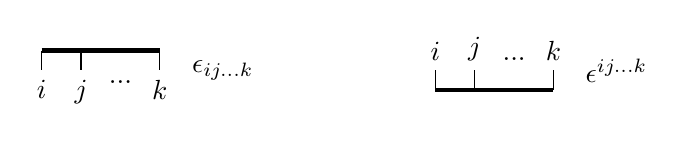
\begin{tikzpicture}
    \coordinate(origin1)at(0,.25);
    \coordinate(origin2)at(5,-.25);
    \draw[ultra thick]
        (origin1)--++(1.5,0)
        (origin2)--++(1.5,0)
    ;
    \draw
        (origin1)--++(0,-.25)
        node[anchor=north]{$i$}
        ++(.5,.25)--++(0,-.25)
        node[anchor=north]{$j$}
        ++(.5,0)node[anchor=north]{$...$}
        ++(.5,.25)--++(0,-.25)
        node[anchor=north]{$k$}
        ++(.8,0)node[anchor=center]{$\epsilon_{ij...k}$}
    ;
    \draw
        (origin2)--++(0,.25)
        node[anchor=south]{$i$}
        ++(.5,-.25)--++(0,.25)
        node[anchor=south]{$j$}
        ++(.5,0)node[anchor=south]{$...$}
        ++(.5,-.25)--++(0,.25)
        node[anchor=south]{$k$}
        ++(.8,0)node[anchor=center]{$\epsilon^{ij...k}$}
    ;
\end{tikzpicture}
